\chapter{Test de convergence}
\section{Curl}
Au vu des problèmes concernant l'erreur des modes propres ($||\rott\bm{g}-\lambda\bm{g}||$), j'ai testé la convergence de l'opérateur rotationnel dans différents espaces. Pour ce faire, j'ai utilisé une fonctions $f$ dont je peux connaître le rotationnel et le rotationnel du rotationnel facilement, j'ai donc essayé avec la fonction :
\[ \bm{f}=\left(\begin{aligned}
\cos(y)+\sin(z)\\
\cos(x)+\sin(z)\\
\sin(xy)
\end{aligned}\right)\text{, }
\rot\bm{f}=\left(\begin{aligned}
x\cos(xy)-\cos(z)\\
\cos(z)-y\cos(xy)\\
\sin(y)-\sin(x)
\end{aligned}\right)\text{, }
\rott\bm{f}=\left(\begin{aligned}
\cos(y)+\sin(z)\\
\cos(x)+\sin(z)\\
(x^2+y^2)\sin(xy)
\end{aligned}\right) \]
Ces fonctions sont entrées comme une option :\\
\lstinputlisting[firstline=20,lastline=22]{../../src/po_app.cfg}
Avec les éléments de Lagrange, l'interpolation est implémenté, je peux donc initialiser directement un vecteur avec cette expression :
\lstinputlisting[linerange={exacte}]{../../src/testCurl.cpp}
Cependant, avec les éléments de Nedelec, l'interpolation n'étant pas encore implémenté, je dois résoudre un autre système pour projeter cette expression :
\lstinputlisting[linerange={Nedelec}]{../../src/testCurl.cpp}
Afin de vérifier les opérateurs, je dois résoudre deux systèmes avec le même membre de gauche, une matrice de masse :\\
\lstinputlisting[linerange={masse}]{../../src/testCurl.cpp}
Le rotationnel est stocké dans $cu$ :\\
\lstinputlisting[linerange={curl}]{../../src/testCurl.cpp}
Puis, je résous encore une fois le même système, avec juste le membre de droite modifié pour appliquer le rotationnel au rotationnel :\\
\lstinputlisting[linerange={curl2}]{../../src/testCurl.cpp}
Enfin, je calcule la norme de l'erreur entre ces résultats et les fonctions passées en option :\\
\lstinputlisting[linerange={erreur}]{../../src/testCurl.cpp}


On peut voir dans la figure \ref{testCVCurl} les résultats de ce test par rapport à différentes tailles de maillage et différents espaces.\\
Les figures \ref{curlO2H1} et \ref{curl2O2H1} montrent la convergence pour l'opérateur $\rot$ et $\rott$ avec des éléments de Lagrange d'ordre 2. On peut voir que la convergence du rotationnel est en $O(h)$, tandis que celle de $\rott$ est plus aléatoire mais tend quand même à baisser.\\
Les figures \ref{curlO3H1} et \ref{curl2O3H1} montrent la convergence pour l'opérateur $\rot$ et $\rott$ avec des éléments de Lagrange d'ordre 3. Après avoir atteint une taille de maille de 0.12, l'erreur de l'opérateur $\rot$ est aussi en $O(h)$. Celle de l'opérateur $\rott$ est minimale pour une taille de maille de 0.2, cependant, le nombre de degré de liberté nécessaire m'a empêché d'avoir des résultats qui sont représentatifs.\\
Les figures \ref{curlNed} et \ref{curl2Ned} montrent la convergence pour l'opérateur $\rot$ et $\rott$ avec des éléments de Nedelec. Si l'erreur de l'opérateur $\rot$ diminue comme souhaité, le rotationnel du rotationnel diverge complètement.\\
\begin{figure}[H]
\makebox[\textwidth][c]{
  \subfloat[$\rot$ avec Lagrange d'ordre 2]{\label{curlO2H1}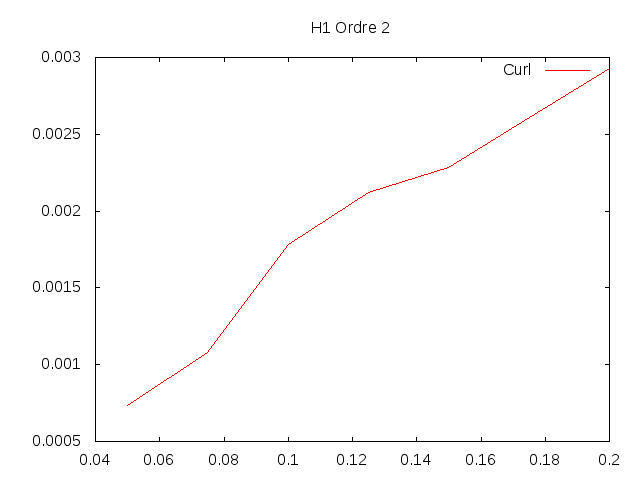
\includegraphics[scale=0.5]{curlO2H1}}\ 
  \subfloat[$\rott$ avec Lagrange d'ordre 2]{\label{curl2O2H1}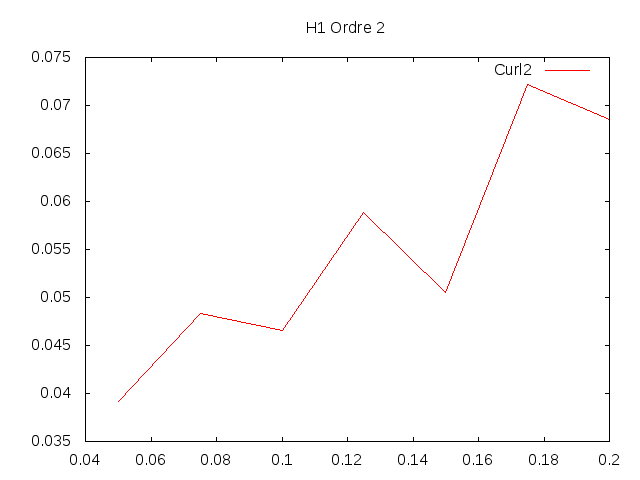
\includegraphics[scale=0.5]{curl2O2H1}}
}\\
\makebox[\textwidth][c]{
  \subfloat[$\rot$ avec Lagrange d'ordre 3]{\label{curlO3H1}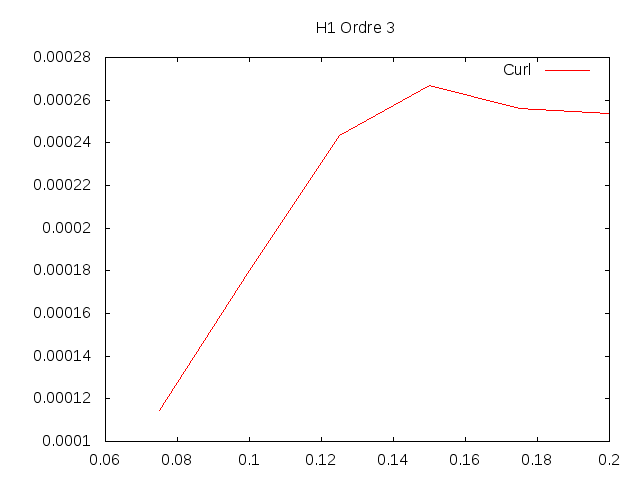
\includegraphics[scale=0.5]{curlO3H1}}\ 
  \subfloat[$\rott$ avec Lagrange d'ordre 3]{\label{curl2O3H1}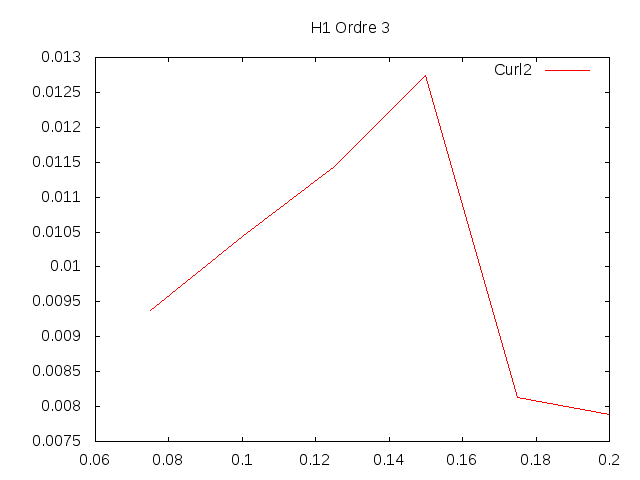
\includegraphics[scale=0.5]{curl2O3H1}}
}\\
\makebox[\textwidth][c]{
  \subfloat[$\rot$ avec Nedelec]{\label{curlNed}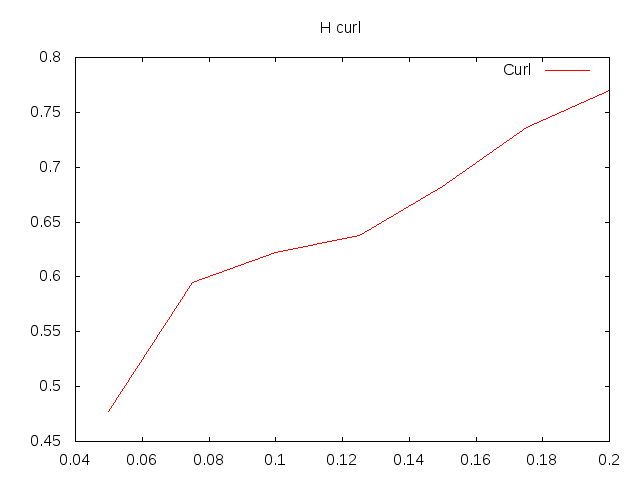
\includegraphics[scale=0.5]{curlNed}}\ 
  \subfloat[$\rott$ avec Nedelec]{\label{curl2Ned}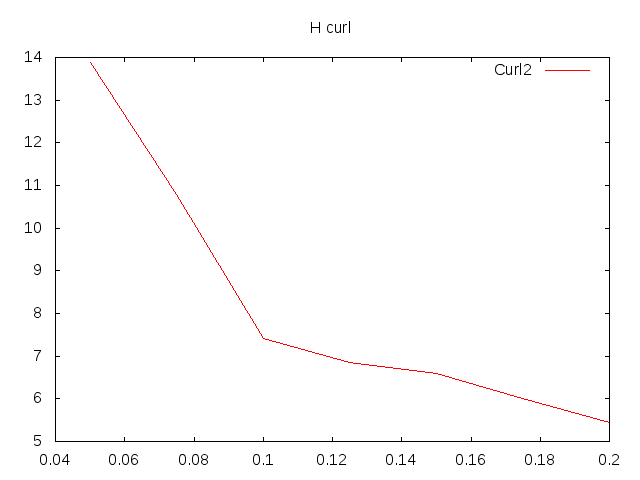
\includegraphics[scale=0.5]{curl2Ned}}
}
\caption{Tests de convergence}
\label{testCVCurl}
\end{figure}

\section{Laplacien}
\subsection{Opérateur} \label{testLapOp}
J'ai aussi vérifier l'opérateur laplacien de la même manière. Comme le laplacien vectoriel est un vecteur composé de laplacien scalaire, je me suis restreint à vérifier ce dernier.\\
Je résous donc deux systèmes, l'un pour trouver le gradient du champ scalaire, qui est un champ vectoriel :\\
\lstinputlisting[linerange={sysGrad,rhsGrad}]{../../src/testgrad.cpp}
Et l'autre pour trouver la divergence d'un champ vectoriel, qui est un champ scalaire et qui est égal au laplacien recherché :\\
\lstinputlisting[linerange={sysDiv,rhsDiv}]{../../src/testgrad.cpp}
Une autre manière de procéder est de prendre la trace de la matrice hessienne, cela à l'avantage de ne nécessiter qu'un seul système à résoudre :\\
\lstinputlisting[linerange={sysHess,rhsHess}]{../../src/testgrad.cpp}

Les différentes erreurs sont présentées dans la figure \ref{testCVLap}.\\
On peut voir que même si les erreurs sont faibles, elles ne tendent pas forcément vers 0, que ce soit avec des éléments de Lagrange d'ordre 2 ou 3, ou en utilisant la divergence du gradient ou la trace de la matrice hessienne.\\
\begin{figure}[H]
\makebox[\textwidth][c]{
  \subfloat[$\div\grad$ avec Lagrange d'ordre 2]{\label{graddivO2}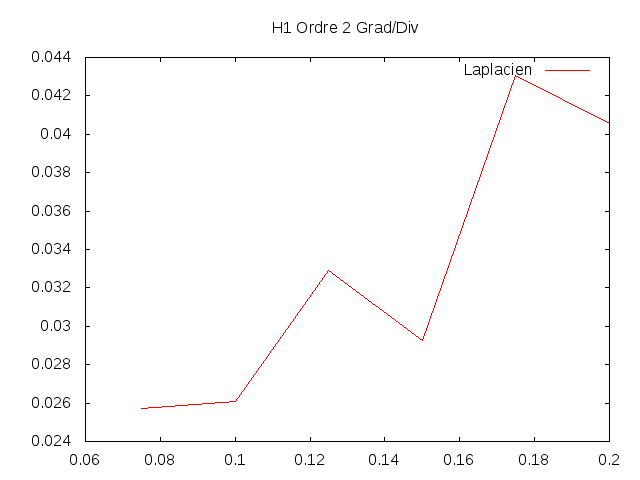
\includegraphics[scale=0.5]{Lap2}}\ 
  \subfloat[$Trace(Hess)$ avec Lagrange d'ordre 2]{\label{hessO2}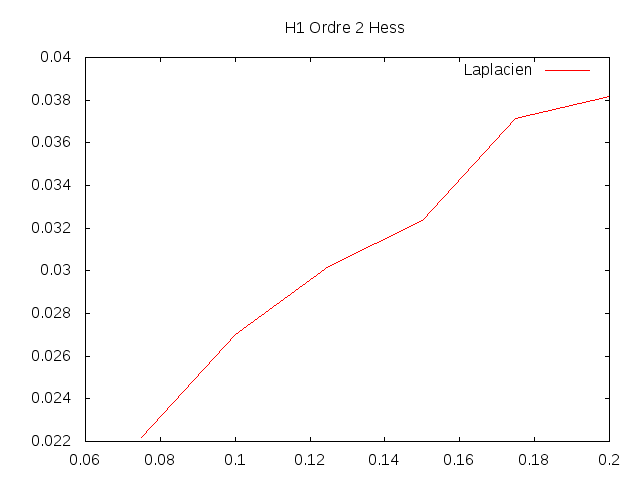
\includegraphics[scale=0.5]{Hess2}}
}\\
\makebox[\textwidth][c]{
  \subfloat[$\div\grad$ avec Lagrange d'ordre 3]{\label{graddivO3}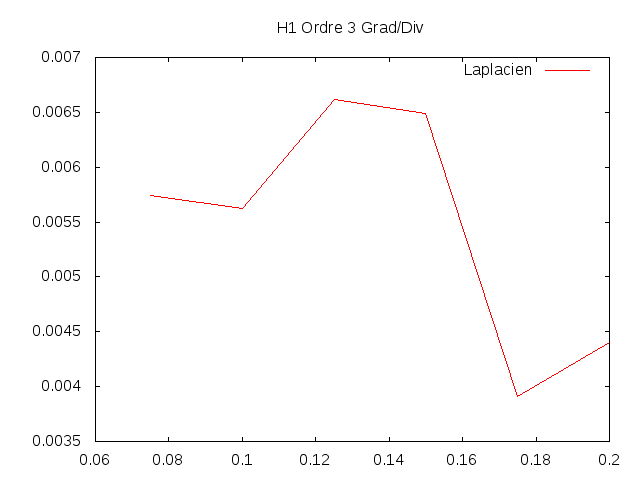
\includegraphics[scale=0.5]{Lap3}}\ 
  \subfloat[$Trace(Hess)$ avec Lagrange d'ordre 3]{\label{hessO3}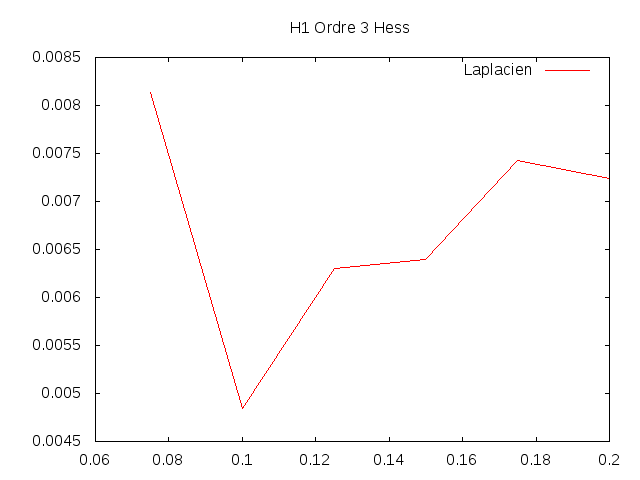
\includegraphics[scale=0.5]{Hess3}}
}
\caption{Tests de convergence}
\label{testCVLap}
\end{figure}

\subsection{Problème aux valeurs propres}
J'ai ensuite cherché à résoudre un problème au valeurs propres de l'opérateur $-\laplace$ scalaire avec des conditions de Dirichlet aux bords.\\
\lstinputlisting[firstline=82,lastline=95]{../../src/testgrad.cpp}

Une fois ce problème résolut, j'ai calculé de la même manière que précédemment le laplacien de chaque vecteur propre. Puis j'ai comparé ce champ scalaire au mode propre multiplié par la valeur propre associée. :\\
\lstinputlisting[firstline=136,lastline=137]{../../src/testgrad.cpp}

Les erreurs sont de l'ordre de la dizaine. La différence entre les résultats de la section \ref{testLapOp} est certainement lié à la régularité des fonctions utilisées pour tester l'opérateur, plus grande que celle des fonctions propres.\\
Une solution serait d'utiliser des éléments de Raviart-Thomas.


%%% Local Variables:
%%% TeX-master: "../report.tex"
%%% eval: (flyspell-mode 1)
%%% ispell-local-dictionary: "french"
%%% End:
